% ====================================================================
% graphite_ica_ch1_v8-03.tex — Chapter 1 (v8-03: 교과서 확장판, 유도 과정 포함)
%   v7-11 배치·결과 박스·식별자·부호·표 보존 + 11개 결과식 유도 단계 전부 복원.
%   신규 그림: g(xi) 이중웰, 플럭스 교차(정지점 유도), 지수 커널 기억(꼬리 유도).
%   build: xelatex -interaction=nonstopmode (2-pass, kotex 한글).
% ====================================================================
\documentclass[11pt,a4paper]{article}
\usepackage[margin=22mm]{geometry}
\usepackage{kotex}
\setmonofont{D2Coding}[Scale=MatchLowercase]
\usepackage{amsmath,amssymb,mathtools,bm}
\usepackage{booktabs,longtable,array}
\usepackage{enumitem}
\usepackage{amsthm}
\usepackage{hyperref}
\usepackage{fancyhdr}
\usepackage{lastpage}
\usepackage{setspace}
\usepackage{tikz}
\usetikzlibrary{positioning,arrows.meta,calc,fit,backgrounds}
\setstretch{1.12}
\setlength{\parskip}{0.45em}\setlength{\parindent}{0pt}\setlength{\headheight}{14pt}
\setlength{\emergencystretch}{2em}
\hypersetup{colorlinks=true, linkcolor=blue, urlcolor=blue, citecolor=blue,
  pdftitle={흑연 음극 dQ/dV 이론: 유도 과정 포함 교과서 확장판 — Chapter 1 (v8)}}
\pagestyle{fancy}\fancyhf{}
\lhead{흑연 음극 $dQ/dV$ 이론 — Ch.1 (v8, 유도 포함 교과서판)}\rhead{\thepage/\pageref{LastPage}}
\renewcommand{\headrulewidth}{0.4pt}

\newtheorem*{keybox}{핵심}
\newtheorem*{codebox}{코드 대응}
\newtheorem*{signbox}{부호 검산}
\newtheorem*{verifybox}{검산}
\newtheorem*{derivbox}{유도}

\newcommand{\dd}{\mathrm{d}}
\newcommand{\eff}{\mathrm{eff}}
\newcommand{\eq}{\mathrm{eq}}
\newcommand{\app}{\mathrm{app}}
\newcommand{\cell}{\mathrm{cell}}
\newcommand{\bg}{\mathrm{bg}}
\newcommand{\rxn}{\mathrm{rxn}}
\newcommand{\dis}{\mathrm{dis}}
\newcommand{\chg}{\mathrm{chg}}
\newcommand{\hys}{\mathrm{hys}}
\newcommand{\work}{\mathrm{work}}
\newcommand{\rep}{\mathrm{rep}}
\newcommand{\sstat}{\mathrm{ss}}
\newcommand{\code}[1]{\texttt{#1}}

\renewcommand{\theequation}{1.\arabic{equation}}
\renewcommand{\thesection}{1.\arabic{section}}
\title{\textbf{\LARGE Chapter 1}\\[0.35em]\Large 흑연 음극 $dQ/dV$ 이론: 유도 과정 포함 교과서 확장판}
\author{}
\date{}

\makeatletter
\renewcommand*\l@section[2]{%
  \ifnum \c@tocdepth >\z@
    \addpenalty\@secpenalty
    \addvspace{1.0em \@plus\p@}%
    \setlength\@tempdima{2.3em}%
    \begingroup
      \parindent \z@ \rightskip \@pnumwidth
      \parfillskip -\@pnumwidth
      \leavevmode \bfseries
      \advance\leftskip\@tempdima
      \hskip -\leftskip
      #1\nobreak\hfil
      \nobreak\hb@xt@\@pnumwidth{\hss #2\kern-\p@\kern\p@}\par
    \endgroup
  \fi}
\renewcommand*\l@subsection{\@dottedtocline{2}{2.3em}{3.2em}}
\makeatother

\begin{document}
\maketitle

% ====================================================================
\section*{서론 — 이 문건이 따라가는 것}
\addcontentsline{toc}{section}{서론}
% ====================================================================
리튬이온전지 흑연 음극의 incremental capacity analysis(ICA)는 충방전 곡선 $Q(V)$ 의 미분
$\dd Q/\dd V$ 를 본다 \cite{bloom2005,dubarry2012}. 흑연은 staging 상전이(stage
$4\!\to\!3\!\to\!2\mathrm L\!\to\!2\!\to\!1$)를 거치며 \cite{dahn1991,ohzuku1993}, 각 전이 전위에서
두 상이 공존하면 전위가 거의 평탄해 좁은 $\dd V$ 에 큰 $\dd Q$ 가 몰려 $\dd Q/\dd V$ 가 치솟는다.

본 문건은 이 곡선을 \emph{한 번 그리는 계산}을 그대로 따라간다. 계산은 구현 \code{Anode\_Fit\_v11\_final.py}
의 메서드 \code{dqdv} 한 번 호출이며, 그 내부는 아홉 단계 $\mathrm N0\!\to\!\mathrm N9$ 를 순서대로 밟는다
(그림~\ref{fig:spine}). 각 절은 그 한 단계에서 코드가 평가하는 물리식을, 그 단계를 이해하는 데 필요한 만큼만
유도한다 — 곡선에 들어가지 않는 일반론은 결과식이 쓰이는 한에서만 최소로 인용한다. 도착점은 한 줄 합산식과,
``이 문건만 보고 같은 곡선을 재현하는 코드를 짤 수 있다''는 실행 가능성이다.

\textbf{v8 확장판의 목적.} v7 계열은 결과 박스를 옳게 제시하되 중간 유도를 압축했다 — 예컨대
spinodal gap, logistic 등온선, $L_q$ 의 지수 표현을 ``대입하면 닫힌다''는 한 줄 점프로 처리했다.
본 v8 문건은 그 열한 개 결과식 각각의 유도 사슬을 (a) 출발 전제 → (b) 적용 연산 → (c) 중간식 →
(d) 결과 박스 네 단계로 명시해, 학부 수준에서 손으로 따라갈 수 있는 교과서판을 만든다.

\textbf{관측.}
\begin{quote}\itshape
$\dd Q/\dd V$ 상전이 peak 의 위치$\cdot$너비$\cdot$높이는 (a) 온도 $T$, (b) 극판 전위, (c) C-rate(전류)
세 가지에 따라 변한다. 저온$\cdot$고율일수록 peak 의 꼬리가 길어져 다음 peak 와 겹치고, 같은 전이가 충전과 방전에서
서로 다른 전위에 peak 를 남기며(충방전 히스테리시스), 이 갈림에는 전류를 $0$ 으로 줄여도 사라지지 않는 성분이 있다.
\end{quote}

세 인자는 모두 하나의 속도식 $k\simeq k_0\exp[-\Delta G_a/RT]$ 의 서로 다른 자리로 들어온다 — 온도는 지수의 분모,
전위는 장벽 $\Delta G_a$ 자체, C-rate 는 요구 속도와 공급 속도의 경쟁이다. 코드 진행이 이 세 갈래를 차례로 닫는다.

\begin{figure}[t]
\centering
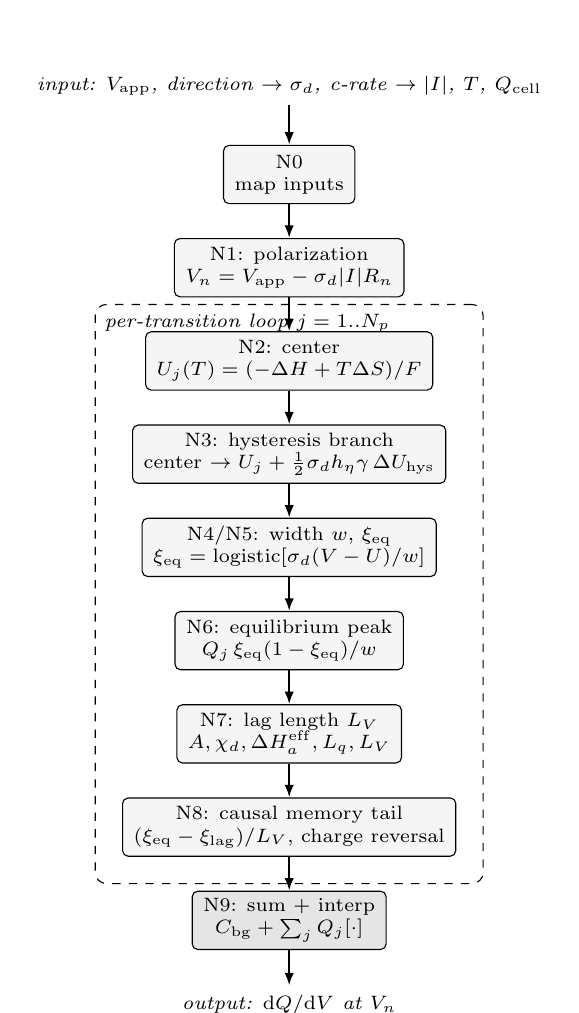
\begin{tikzpicture}[
  node distance=4.3mm and 5.5mm,
  stage/.style={draw,rounded corners=2pt,minimum height=7.4mm,inner xsep=4pt,inner ysep=2.5pt,font=\scriptsize,align=center,fill=black!4},
  core/.style={stage,fill=black!10},
  io/.style={font=\scriptsize\itshape,align=center},
  ar/.style={-{Latex[length=1.6mm]},thick}]
% input row
\node[io] (in) {input: $V_\app$, direction $\to\sigma_d$, c-rate $\to|I|$, $T$, $Q_\cell$};
% spine
\node[stage,below=5mm of in] (n0) {N0\\map inputs};
\node[stage,below=of n0] (n1) {N1: polarization\\$V_n=V_\app-\sigma_d|I|R_n$};
\node[stage,below=of n1] (n2) {N2: center\\$U_j(T)=(-\Delta H+T\Delta S)/F$};
\node[stage,below=of n2] (n3) {N3: hysteresis branch\\center $\to U_j+\tfrac12\sigma_d h_\eta\gamma\,\Delta U_\hys$};
\node[stage,below=of n3] (n4) {N4/N5: width $w$, $\xi_\eq$\\$\xi_\eq=\mathrm{logistic}[\sigma_d(V-U)/w]$};
\node[stage,below=of n4] (n6) {N6: equilibrium peak\\$Q_j\,\xi_\eq(1-\xi_\eq)/w$};
\node[stage,below=of n6] (n7) {N7: lag length $L_V$\\$A,\chi_d,\Delta H_a^\eff,L_q,L_V$};
\node[stage,below=of n7] (n8) {N8: causal memory tail\\$(\xi_\eq-\xi_\mathrm{lag})/L_V$, charge reversal};
\node[core,below=of n8] (n9) {N9: sum + interp\\$C_\bg+\sum_j Q_j[\cdot]$};
\node[io,below=4.5mm of n9] (out) {output: $\dd Q/\dd V$ at $V_n$};
\foreach \a/\b in {in/n0,n0/n1,n1/n2,n2/n3,n3/n4,n4/n6,n6/n7,n7/n8,n8/n9,n9/out}
  \draw[ar] (\a) -- (\b);
% per-transition loop bracket
\begin{scope}[on background layer]
\node[draw,dashed,rounded corners,fit=(n2)(n3)(n4)(n6)(n7)(n8),inner sep=3.4mm,label={[font=\scriptsize\itshape,anchor=north west]north west:per-transition loop $j=1..N_p$}] (loop) {};
\end{scope}
\end{tikzpicture}
\caption{한 곡선을 그리는 코드 진행(spine). 외부 실험조건이 \code{curve} facade 에서 $(\sigma_d,|I|,T,Q_\cell)$
로 환산($\mathrm N0$)되어 코어 \code{dqdv} 로 들어가고, 분극으로 내부 전위 $V_n$ 을 얻은 뒤($\mathrm N1$),
전이 $j$ 마다 평형 중심$\cdot$히스 분기$\cdot$폭$\cdot$평형 점유$\cdot$평형 peak$\cdot$지연 길이$\cdot$인과 꼬리를
계산해($\mathrm N2$--$\mathrm N8$) 합산$\cdot$역보간한다($\mathrm N9$). 본 문건의 절 번호가 이 노드 순서다.}
\label{fig:spine}
\end{figure}

\tableofcontents
\newpage

% ====================================================================
\section{기호와 규약, 실험조건 매핑 (N0)}\label{sec:notation}
% ====================================================================
계산의 진입점은 facade \code{curve}$(V_\app,\text{direction},\text{c\_rate},Q_\cell,T)$ 이고, 그 첫 일은 실험조건을
코어 \code{dqdv} 의 모델 입력으로 환산하는 것이다 — 이것이 노드 $\mathrm N0$ 다. 방향 문자열은 방향 부호 $\sigma_d$ 로,
C-rate 는 전류 크기 $|I|$ 로 바뀐다:
\begin{equation}
\sigma_d=\begin{cases}+1 & \text{방전(discharge)}\\ -1 & \text{충전(charge)}\end{cases},
\qquad
|I|=\text{c\_rate}\cdot Q_\cell\quad(\text{또는 }I_\mathrm{abs}\text{ 직접 지정}).
\label{eq:n0map}
\end{equation}
방향 부호의 작용처는 셋 — 분극 부호($\mathrm N1$), 분기 중심 선택($\mathrm N3$), 꼬리 지지 방향($\mathrm N8$) — 이며,
평형 종 자체는 방향 불변이다.

\textbf{전이 인덱스.} $j=1,\dots,N_p$($N_p\approx3$--$4$). 전이 $j$ 의 진행률 $\xi_j$(방전 시 $0\to1$ 로 증가,
곧 탈리튬화 진행), 용량 가중 $Q_j$.

\textbf{부호 규약(★최우선 결함 클래스).} 전위는 흑연 음극 반쪽전지 전위(vs Li/Li$^+$)다. 방향 부호 $\sigma_d=\pm1$
(방전 $+1$/충전 $-1$)이 코드의 \code{s} 인자이며, 평형 점유 $\xi_\eq=\mathrm{logistic}[\sigma_d(V-U)/w]$ 에서 방전
($\sigma_d=+1$)은 $V\!\uparrow\Rightarrow\xi_\eq\!\uparrow$(전위를 올리면 탈리튬화).

\begin{longtable}{p{0.17\textwidth} p{0.16\textwidth} p{0.585\textwidth}}
\toprule 기호(코드 식별자) & 단위 & 의미 \\ \midrule \endhead
\multicolumn{3}{l}{\emph{— 실험조건$\cdot$방향(N0$\cdot$N1) —}}\\
$\sigma_d$ (\code{s},\,\code{sigma\_d}) & --- & 방향 부호 — 방전 $+1$/충전 $-1$ \\
$|I|$ (\code{I\_abs}) & A & 전류 크기 $=$ c\_rate$\cdot Q_\cell$ \\
$Q_\cell$ (\code{Q\_cell}) & C & 셀 용량(전하) \\
$T$ (\code{T}) & K & 온도 — 스칼라 또는 $V_\app$ 길이 배열($T(V)$ 비등온) \\
$R_n$ (\code{Rn}) & $\Omega$ & 음극 lumped 분극 저항 \\
$V_\app$ (\code{V\_app}) & V & 인가(측정) 전위 격자 \\
$V_n$ & V & 내부(열역학) 전위 $=V_\app-\sigma_d|I|R_n$ \\
\multicolumn{3}{l}{\emph{— 평형 중심$\cdot$폭$\cdot$점유(N2$\cdot$N4$\cdot$N5) —}}\\
$U_j(T)$ (\code{U},\,\code{func\_U\_j}) & V & 전이 $j$ 평형 중심 전위 $=(-\Delta H_\rxn+T\Delta S_\rxn)/F$ \\
$\Delta H_{\rxn,j},\Delta S_{\rxn,j}$ & {\footnotesize J/mol;\,J/(mol\,K)} & 삽입 반응 엔탈피$\cdot$엔트로피 \\
$n_j$ (\code{n}) & --- & 폭 다중도($w=n_jRT/F$) \\
$w_j$ (\code{func\_w}/\code{func\_w\_eff}) & V & 전이 폭 척도 $=n_jRT/F$ \\
$\xi_{\eq,j}$ (\code{func\_ksi\_eq}) & --- & 평형 진행률(logistic) \\
$Q_j$ (\code{Q}) & C & 전이 $j$ 용량 가중 \\
$C_\bg$ (\code{Cbg}) & C/V & 배경 미분용량 \\
\multicolumn{3}{l}{\emph{— 히스테리시스 분기(N3) —}}\\
$\Omega_j$ (\code{Omega}) & J/mol & 정규용액 상호작용 에너지 \\
$\gamma_j$ (\code{gamma}) & --- & 분기 축소 인자 $0\le\gamma_j\le1$ \\
$\Delta U_j^\hys$ (\code{func\_dU\_hys}) & V & spinodal 상한 분기 gap \\
$h_{\eta,j}$ (\code{h\_eta}) & --- & 부분 cycle 인자(기본 $1$) \\
$U_j^{\,d}$ (\code{center},\,\code{func\_U\_branch}) & V & 방향별 분기 중심 \\
\multicolumn{3}{l}{\emph{— 동역학 꼬리(N7$\cdot$N8) —}}\\
$\chi$ (\code{chi},\,\code{x}) & --- & 전이상태 분율 위치(전달 계수) \\
$\chi_d$ (\code{func\_chi\_d}) & --- & 방향별 전달 계수 — 방전 $\chi$/충전 $1-\chi$ \\
$\mathcal A$ (\code{A}) & J/mol & 꼬리 컷점 affinity $=\min(z_\mathrm{cut}n_jRT,\,A_\mathrm{cap}RT)$ \\
$\Delta H_{a,j},\Delta S_{a,j}$ & {\footnotesize J/mol;\,J/(mol\,K)} & 활성화 엔탈피$\cdot$엔트로피 \\
$\Delta H_{a,j}^\eff$ (\code{func\_dH\_a\_eff}) & J/mol & 유효 장벽 $=\Delta H_a-\chi_d\Omega$ \\
$L_{q,j}$ (\code{func\_L\_q}) & --- & 용량축 지연 길이 \\
$L_{V,j}$ (\code{lag\_len\_V}) & V & 전압축 지연 길이 $=|\dd V/\dd q|_{q_a}L_{q,j}$ \\
$z_\mathrm{cut}$ (\code{z\_cut}) & --- & 컷 affinity 의 $z=\mathcal A/(n_jRT)$(기본 $4.357$) \\
$A_\mathrm{cap}$ (\code{A\_cap\_RT}) & --- & 컷 affinity 상한 배수(기본 $4.0$) \\
$\xi_{\mathrm{lag},j}$ (\code{occ\_lagged}) & --- & 인과 저역통과된 진행률 \\
\multicolumn{3}{l}{\emph{— 상수 —}}\\
$R,F,k_B,h$ & {\footnotesize J/(mol\,K), C/mol, J/K, J\,s} & 기체상수, Faraday, Boltzmann, Planck \\
\bottomrule
\end{longtable}

흑연 staging 의 갤러리 채움을 그림~\ref{fig:staging} 에 둔다.

\begin{figure}[t]
\centering
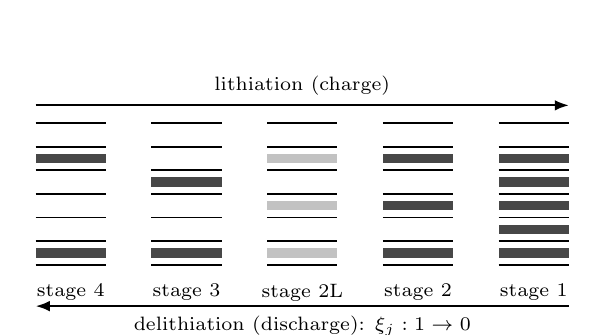
\begin{tikzpicture}[x=1.05cm,y=0.5cm,
  lab/.style={font=\scriptsize,align=center}]
\def\colw{0.85}
\foreach \x/\name in {0/{stage 4}, 1.4/{stage 3}, 2.8/{stage 2L}, 4.2/{stage 2}, 5.6/{stage 1}}{
  \draw[semithick] (\x,0)--(\x+\colw,0);
  \foreach \k in {1,2,3,4,5,6}{\draw[semithick] (\x,0.6*\k)--(\x+\colw,0.6*\k);}
  \node[lab,below] at (\x+\colw/2,-0.25) {\name};
}
% stage 4: every 4th gallery filled
\foreach \k in {1,5}{\fill[black!72] (0,0.6*\k-0.42) rectangle (0+\colw,0.6*\k-0.18);}
% stage 3: every 3rd
\foreach \k in {1,4}{\fill[black!72] (1.4,0.6*\k-0.42) rectangle (1.4+\colw,0.6*\k-0.18);}
% stage 2L: every 2nd, light
\foreach \k in {1,3,5}{\fill[black!24] (2.8,0.6*\k-0.42) rectangle (2.8+\colw,0.6*\k-0.18);}
% stage 2: every 2nd, dark
\foreach \k in {1,3,5}{\fill[black!72] (4.2,0.6*\k-0.42) rectangle (4.2+\colw,0.6*\k-0.18);}
% stage 1: all galleries
\foreach \k in {1,2,3,4,5}{\fill[black!72] (5.6,0.6*\k-0.42) rectangle (5.6+\colw,0.6*\k-0.18);}
\draw[-{Latex[length=1.8mm]},thick] (0,4.05)--(6.45,4.05) node[pos=0.5,above,font=\scriptsize] {lithiation (charge)};
\draw[{Latex[length=1.8mm]}-,thick] (0,-1.05)--(6.45,-1.05) node[pos=0.5,below,font=\scriptsize] {delithiation (discharge): $\xi_j:1\to0$};
\end{tikzpicture}
\caption{흑연 staging 의 갤러리 채움 도식(v7-11 유래). 수평선이 그래핀 층, 음영 띠가 리튬이 든 층간 갤러리다.
각 stage 전이가 $\dd Q/\dd V$ 에 peak 하나를 남긴다. stage $2\mathrm L$ 은 면내 질서가 풀린 단계라 옅게 표시했다.}
\label{fig:staging}
\end{figure}

% ====================================================================
\section{분극 — 측정 전위에서 내부 전위로 (N1)}\label{sec:pol}
% ====================================================================
코어 \code{dqdv} 의 첫 식은 분극을 벗기는 환산이다. 관측은 유한 전류에서 이루어지므로 측정 전위 $V_\app$ 에는 셀의
직렬 저항을 통과한 IR 분극이 실려 있고, 평형 열역학이 사는 전위는 그 분극을 벗긴 내부 전위 $V_n$ 이다.

\subsection{분극 부호 — 방향이 결정한다}
전류 크기 $|I|$ 가 lumped 저항 $R_n$ 을 통과하며 만드는 전위 강하가 $|I|R_n$ 이고, 그 부호는 전류 방향이 정한다.
방전($\sigma_d=+1$)은 음극에서 산화(탈리튬화)가 일어나는 방향이라 측정 전위가 내부 전위보다 분극만큼 \emph{높게}
관측되므로, 내부 전위는 그만큼 낮춰 읽어야 한다. 충전($\sigma_d=-1$)은 부호가 반대다. 두 경우를 한 식으로 묶으면
\begin{equation}
\boxed{\;V_n\;=\;V_\app\;-\;\sigma_d\,|I|\,R_n\;.}
\label{eq:vn}
\end{equation}
이것이 코드의 \code{V\_n = V\_in - sigma\_d * I\_abs * self.Rn} 한 줄이다. 부호 약속을 식으로 확인하면 —
방전에서 $V_n=V_\app-|I|R_n<V_\app$(측정이 내부보다 높음), 충전에서 $V_n=V_\app+|I|R_n>V_\app$ — 이며,
$|I|\to0$ 또는 $R_n=0$ 에서 $V_n=V_\app$ 로 두 전위가 일치한다.

\subsection{작업 격자 — 꼬리가 들어올 여유}
이후 모든 전이 계산은 $V_n$ 을 직접 쓰지 않고, $V_n$ 의 범위를 양쪽으로 넓힌 균일 \emph{작업 격자} $V_\work$ 위에서
이루어진다. $v_\mathrm{lo}=\min V_n$, $v_\mathrm{hi}=\max V_n$, $\Delta v=v_\mathrm{hi}-v_\mathrm{lo}$ 로
\begin{equation}
V_\work=\mathrm{linspace}\big(v_\mathrm{lo}-p_\mathrm{lo}\,\Delta v,\;
v_\mathrm{hi}+p_\mathrm{hi}\,\Delta v,\;n_\work\big),
\qquad \Delta_\mathrm{grid}=V_{\work,1}-V_{\work,0},
\label{eq:vwork}
\end{equation}
패딩 $p_\mathrm{lo}=p_\mathrm{hi}=0.15$, 점 수 $n_\work=\max(2048,\,2\,|V_n|)$ 이다.

\begin{keybox}
\textbf{세 전위.} $V_\app$(측정)$\cdot$$V_n$(내부, 식~\eqref{eq:vn})$\cdot$$V_\work$(계산 격자, 식~\eqref{eq:vwork})는
지위가 다르다. 다음 절부터 평형$\cdot$동역학은 $V_\work$ 위에서 풀고, 출력만 $V_n$ 으로 되돌린다.
\end{keybox}

% ====================================================================
\section{평형 중심 $U_j(T)$ — 열역학에서 (N2)}\label{sec:center}
% ====================================================================
전이 루프 안의 첫 물리량은 전이 $j$ 의 평형 중심 전위 $U_j(T)$ 다. 이 절은 Gibbs 자유에너지에서 출발해,
삽입 반응 전기화학 평형을 거쳐, 온도 의존 환산식이 닫히는 전 과정을 단계별로 전개한다.

\subsection{출발: $G$, $\mu$, 평형 조건}

\textbf{(a) 출발 전제.} 등온$\cdot$등압 계(전지)의 자발성과 평형을 판정하는 퍼텐셜은 Gibbs 자유에너지다:
\begin{equation}
G \equiv H - TS.
\label{eq:gibbsdef}
\end{equation}
입자 1몰 변화당 $G$ 변화가 화학퍼텐셜이다:
\begin{equation}
\mu \equiv \frac{\partial G}{\partial n}\bigg|_{T,P}.
\label{eq:mudef}
\end{equation}
두 장소의 $\mu$ 가 일치하는 조건이 입자 교환 평형이다.

\textbf{(b) 삽입 반응과 전기화학 평형.} 흑연 음극의 삽입 반응은
\begin{equation}
\mathrm{Li}^+ + e^- + [\,] \;\rightleftharpoons\; \mathrm{Li}_{(\text{흑연})}
\label{eq:insertion}
\end{equation}
이다. 하전 입자의 값어치에는 전기 일이 더해져 전기화학 퍼텐셜 $\tilde\mu \equiv \mu + zF\phi$ 가 된다
(전자: $z=-1$, Li$^+$: $z=+1$, 삽입 Li: $z=0$). 전극 내부 전위 $\phi$ 와 측정 전위 $V$ 의 상수 차이는
기준 몫으로 흡수하므로 전자 항에 $V$ 를 바로 쓴다. 반응 평형 조건 $\delta G = 0$ 은
\begin{equation}
\tilde\mu_{\mathrm{Li}^+} + \tilde\mu_{e^-} = \tilde\mu_{\mathrm{Li}}
\label{eq:eqbalance}
\end{equation}
이다. 전해질 조성이 운전 중 일정하다면 좌변의 Li$^+$·$e^-$ 항은 온도에서 정해지는 상수 묶음으로 정리되고,
그 상수 묶음을 $sFU$ 로 정의하면($s=+1$, 방전 규약)

\textbf{(c) 중간식 — 상수 묶음 정리.} 좌변 각 항을 전기화학 퍼텐셜로 전개하면
\begin{equation}
\bigl[\mu^0_{\mathrm{Li}^+} + RT\ln a_{\mathrm{Li}^+} + F\phi_\mathrm{elyte}\bigr]
+ \bigl[\mu^0_{e^-} - FV\bigr]
= \mu_{\mathrm{Li}}(\theta_\eq).
\label{eq:eqexpand}
\end{equation}
전해질 항은 상수 $sFU^0 \equiv \mu^0_{\mathrm{Li}^+} + RT\ln a_{\mathrm{Li}^+} + F\phi_\mathrm{elyte} + \mu^0_{e^-}$
로 묶이고, 기준 몫 $\mu^0$(격자기체 식~\eqref{eq:mu} 내 기준)까지 흡수해 $U_j$ 를 재정의하면
\begin{equation}
\mu_{\mathrm{Li}}(\theta_\eq) = \mu^0 - sF(V-U_j)
\label{eq:eqcond}
\end{equation}
형태가 된다. $\Delta G_j \equiv -sFU_j$ 라는 지위 — $U_j$ 가 양이면 $\Delta G_j < 0$, 전이가 자발 진행할
전위가 양의 중심이다.

\textbf{(d) $U_j(T)$ — 온도 환산.} 열역학 항등식 $\Delta G_j = \Delta H_{\rxn,j} - T\Delta S_{\rxn,j}$ 를
$\Delta G_j = -sFU_j$($s=+1$)에 넣고 $U_j$ 로 풀면
\begin{equation}
\boxed{\;U_j(T)\;=\;\frac{-\Delta H_{\rxn,j}+T\,\Delta S_{\rxn,j}}{F}\;.}
\label{eq:Uj}
\end{equation}

\subsection{$U_j(T)$ 해설 및 코드 대응}
부호 — 발열 반응 $\Delta H_\rxn<0$ 이면 분자 $-\Delta H_\rxn>0$ 이 중심을 \emph{올린다}(흡열 아님에 주의).
온도 의존은 $\partial U_j/\partial T=\Delta S_{\rxn,j}/F$ 이고, $|\Delta S_\rxn|\sim$ 수십 J/(mol\,K) 라
$30$ K 창에서 수 mV 규모로 중심이 이동한다.

\begin{codebox}
\textbf{N2.} \code{if 'dH\_rxn' in tr and 'dS\_rxn' in tr: U\_j = func\_U\_j(T\_work, dH\_rxn, dS\_rxn)}
— 배열 $T_\work$ 대응. 없으면 \code{U\_j = float(tr['U'])} 직접. \code{GRAPHITE\_STAGING\_LIT} 의 stage 2$\to$1 은
$\Delta H_\rxn=-13000$ J/mol, $\Delta S_\rxn=-16$ J/(mol\,K) $\Rightarrow$ $U(298)=(13000-298.15\times16)/96485
\approx0.0853$ V(목표 $0.085$ V 정합).
\end{codebox}

% ====================================================================
\section{히스테리시스 분기 중심 (N3)}\label{sec:hys}
% ====================================================================
코드는 평형 중심 $U_j$ 를 곧바로 쓰지 않고, 상호작용 $\Omega_j$ 와 분기 인자 $\gamma_j$ 가 있으면 방향별 분기 중심
$U_j^{\,d}$ 로 옮긴다. 이 절은 상호작용 자유에너지, spinodal 조건, gap 의 닫힌 꼴을 단계별로 전개한다.

\subsection{자유에너지와 spinodal 조건}

\textbf{(a) 출발: 격자기체 자유에너지.} 진행률 $\xi$ 의 자유에너지 밀도는
\begin{equation}
g_j(\xi)=g_j^0+RT\big[\xi\ln\xi+(1-\xi)\ln(1-\xi)\big]+\Omega_j\,\xi(1-\xi).
\label{eq:gxi}
\end{equation}
첫 항은 기준, 둘째 항은 섞임 엔트로피($-TS_\mathrm{mix}$), 셋째 항은 이웃 쌍 상호작용이다
($\Omega_j>0$ 이면 동종 이웃 인력).

그림~\ref{fig:gxi} 는 $\Omega_j>2RT$ 일 때 $g(\xi)$ 가 이중웰(double well)이 됨을 보인다.

\begin{figure}[t]
\centering
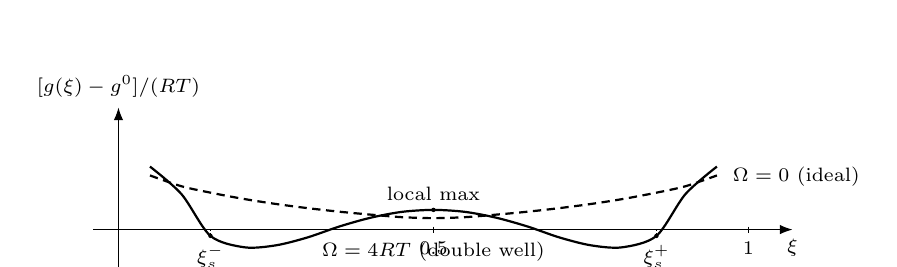
\begin{tikzpicture}[x=8.0cm,y=2.5cm]
% axes
\draw[-{Latex[length=1.6mm]}] (-0.04,0) -- (1.07,0) node[below,font=\scriptsize] {$\xi$};
\draw[-{Latex[length=1.6mm]}] (0,-0.22) -- (0,0.62) node[above,font=\scriptsize] {$[g(\xi)-g^0]/(RT)$};
\foreach \xx in {0.5,1} {\draw (\xx,0.015) -- (\xx,-0.015) node[below,font=\scriptsize] {\xx};}
% Omega=0 (ideal, no double-well): monotone convex — dashed
% g_ideal = xi ln xi + (1-xi)ln(1-xi), max-min ~ 0 to ln2 ~ 0.693, plotted scaled
% approximate: xi*ln(xi)+(1-xi)*ln(1-xi) scaled so center ~ 0, values ~-0.693 to 0
% shift up by 0.35 to keep visible
\draw[densely dashed,thick] plot[smooth] coordinates {
  (0.05,0.275)(0.10,0.22)(0.15,0.185)(0.20,0.155)(0.25,0.13)(0.30,0.109)
  (0.35,0.091)(0.40,0.076)(0.45,0.063)(0.50,0.058)
  (0.55,0.063)(0.60,0.076)(0.65,0.091)(0.70,0.109)(0.75,0.13)
  (0.80,0.155)(0.85,0.185)(0.90,0.22)(0.95,0.275)};
\node[font=\scriptsize,right] at (0.96,0.27) {$\Omega=0$ (ideal)};
% Omega=4RT double well: g = xi*ln(xi)+(1-xi)ln(1-xi) + 4*xi*(1-xi)
% min near xi=0.15 and 0.85, max at xi=0.5
% qualitative: adjusted coordinates
\draw[thick] plot[smooth] coordinates {
  (0.05,0.32)(0.10,0.18)(0.146,-0.032)(0.20,-0.09)(0.25,-0.08)(0.30,-0.04)
  (0.35,0.015)(0.40,0.06)(0.45,0.09)(0.50,0.10)
  (0.55,0.09)(0.60,0.06)(0.65,0.015)(0.70,-0.04)
  (0.75,-0.08)(0.80,-0.09)(0.854,-0.032)(0.90,0.18)(0.95,0.32)};
\fill (0.146,-0.032) circle (0.8pt) node[below,font=\scriptsize] {$\xi_s^-$};
\fill (0.854,-0.032) circle (0.8pt) node[below,font=\scriptsize] {$\xi_s^+$};
\fill (0.50,0.10) circle (0.8pt) node[above,font=\scriptsize] {local max};
\draw[densely dotted] (0.146,0)--(0.146,-0.032);
\draw[densely dotted] (0.854,0)--(0.854,-0.032);
\node[font=\scriptsize] at (0.50,-0.11) {$\Omega=4RT$ (double well)};
\end{tikzpicture}
\caption{격자기체 자유에너지 $g(\xi)$(신규). 파선 $=\Omega=0$ 이상(단조 볼록, 상분리 없음). 실선 $=\Omega=4RT>2RT$
이중웰 — 두 극소 $\xi_s^\pm$ 가 spinodal 점이고(식~\eqref{eq:spinodal}), 가운데 극대가 불안정 영역이다.
$g''=0$ 두 근이 공존 상경계다.}
\label{fig:gxi}
\end{figure}

\textbf{(b) 적용 연산 — $g''=0$.} 식~\eqref{eq:gxi} 를 두 번 미분하면
\begin{equation}
g_j''(\xi) = \frac{RT}{\xi(1-\xi)} - 2\Omega_j.
\label{eq:gpp}
\end{equation}
$g_j''=0$ 을 $\xi$ 에 대해 풀면 $RT/[\xi(1-\xi)]=2\Omega_j$, 즉 $\xi(1-\xi)=RT/(2\Omega_j)$ 다.
$\xi^2-\xi+RT/(2\Omega_j)=0$ 의 근의 공식을 적용하면

\textbf{(c) 중간식 — 근의 공식.}
\begin{equation}
\xi_{s,j}^\pm = \frac{1 \pm \sqrt{1 - 4\cdot RT/(2\Omega_j)}}{2}
= \frac{1 \pm \sqrt{1 - 2RT/\Omega_j}}{2}
= \tfrac12(1\pm u_j),
\label{eq:spinodalderiv}
\end{equation}
$u_j \equiv \sqrt{1-2RT/\Omega_j}$ 라 두면

\textbf{(d) spinodal 결과.}
\begin{equation}
\boxed{\;\xi_{s,j}^\pm=\tfrac12(1\pm u_j),\qquad
u_j\equiv\sqrt{1-\frac{2RT}{\Omega_j}}\quad(\Omega_j>2RT)\;.}
\label{eq:spinodal}
\end{equation}
$u_j$ 가 실수가 되는 조건 $\Omega_j>2RT$ 가 상분리의 문턱이다. 이 문턱이 코드의 명시 분기
\code{if Omega <= 2*R*T: return 0.0} 이다.

\subsection{$\Delta U_j^\hys$ — 두 spinodal 의 전위 차}

\textbf{(a) 출발: 비단조 평형 전위 곡선.} 자유에너지~\eqref{eq:gxi} 에서 나온 평형 전위는
\begin{equation}
V_{\eq,j}(\xi) = U_j + \frac{RT}{sF}\ln\frac{\xi}{1-\xi} + \frac{\Omega_j}{sF}(1-2\xi).
\label{eq:Veq}
\end{equation}
$\Omega_j>2RT$ 면 이 곡선은 비단조이고, 방전과 충전이 각각 다른 극값까지 과주행한다
(그림~\ref{fig:hysloop}).

\textbf{(b) spinodal 대입.} 두 극값 $(V_{\eq,j}^-, V_{\eq,j}^+)$ 를 $\xi_{s,j}^\mp$ 에서 구한다
(방전은 극대 $\xi_s^-$, 충전은 극소 $\xi_s^+$).
$\xi_{s,j}^\pm = \tfrac12(1\pm u_j)$ 를 로그 항에 넣으면:
\begin{equation}
\ln\frac{\xi_{s,j}^+}{1-\xi_{s,j}^+}
= \ln\frac{\tfrac12(1+u_j)}{\tfrac12(1-u_j)}
= \ln\frac{1+u_j}{1-u_j},
\qquad
\ln\frac{\xi_{s,j}^-}{1-\xi_{s,j}^-}
= \ln\frac{1-u_j}{1+u_j} = -\ln\frac{1+u_j}{1-u_j}.
\label{eq:logitspinodal}
\end{equation}
즉 두 끝점의 로그 몫은 서로 역수 관계다. 또한
$(1-2\xi_{s,j}^-) = 1-2\cdot\tfrac12(1-u_j) = +u_j$ 이고
$(1-2\xi_{s,j}^+) = -u_j$ 이다.

\textbf{(c) 중간식 — 전위 차.} 방전 극대 $V_{\eq}^-$ 에서 충전 극소 $V_{\eq}^+$ 를 뺀다
($s=+1$):
\begin{align}
V_{\eq,j}^- - V_{\eq,j}^+
&= \frac{RT}{F}\Bigl[\ln\frac{1-u_j}{1+u_j} - \ln\frac{1+u_j}{1-u_j}\Bigr]
+ \frac{\Omega_j}{F}\bigl[u_j - (-u_j)\bigr] \notag\\
&= \frac{RT}{F}\bigl[-2\ln\tfrac{1+u_j}{1-u_j}\bigr] + \frac{2\Omega_j}{F}u_j.
\label{eq:Vdiff}
\end{align}
$\ln\tfrac{1+u}{1-u} = 2\,\mathrm{artanh}\,u$ 이므로

\textbf{(d) $\Delta U_j^\hys$ 닫힌 꼴.}
\begin{equation}
\boxed{\;\Delta U_j^\hys
=\frac{2}{F}\Big[\Omega_j\,u_j-2RT\,\mathrm{artanh}\,u_j\Big],
\qquad u_j=\sqrt{1-\frac{2RT}{\Omega_j}}\;.}
\label{eq:dUhys}
\end{equation}
이것이 \code{func\_dU\_hys(T, Omega)} 의 \code{(2/F)*(Omega*u - 2*R*T*arctanh(u))} 이며,
$\Omega\le2RT$ 면 $0$ 을 반환한다. 부호 — 극대 $>$ 극소라 $\Delta U_j^\hys\ge0$,
$\Omega_j\to2RT^+$ 에서 $u_j\to0$, $\Delta U_j^\hys\to0$ 으로 연속이다.

\subsection{방향별 분기 중심 $U_j^{\,d}$}
두 spinodal 끝점의 평균은 로그 몫 합과 $(1-2\xi)$ 몫 합이 둘 다 $0$ 이라 정확히 $U_j$ 다 —
분기는 $U_j$ 대칭이다. 실측 분기 중심을 방향별 한 자유도로 적으면
\begin{equation}
\boxed{\;U_j^{\,d}\;=\;U_j\;+\;\tfrac12\,\sigma_d\,h_{\eta,j}\,\gamma_j\,\Delta U_j^\hys\;.}
\label{eq:Ubranch}
\end{equation}
이것이 \code{func\_U\_branch(T, U\_j, Omega, gamma, sigma\_d, h\_eta)} 다. 부호 —
방전($\sigma_d=+1$)은 중심을 $+$ 쪽, 충전($\sigma_d=-1$)은 $-$ 쪽으로 옮겨 $U_j^\dis>U_j^\chg$.

코드는 전이당 상수 shift 만 필요하므로 $U_j=0$ 로 넣어 shift 를 얻고, 배열 중심 $U_j$ 에 더한다:
\begin{equation}
\mathrm{center}=
\begin{cases}
U_j+\tfrac12\sigma_d h_{\eta,j}\gamma_j\Delta U_j^\hys(T_\rep) & \gamma_j\ne0 \text{ 이고 } \Omega_j>0\\[2pt]
U_j & \text{그 외(분기 없음)}.
\end{cases}
\label{eq:center}
\end{equation}

\begin{figure}[t]
\centering
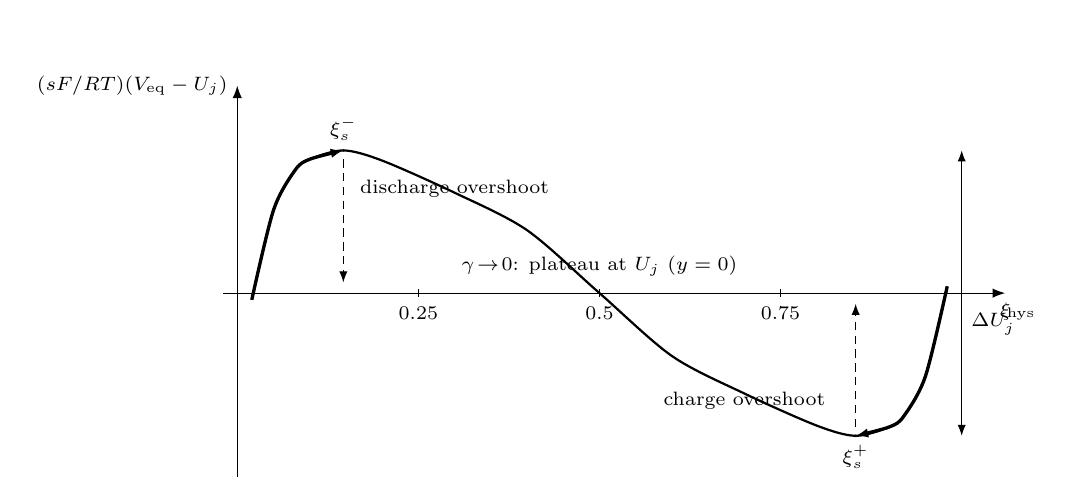
\begin{tikzpicture}[x=9.2cm,y=1.7cm]
\draw[-{Latex[length=1.6mm]}] (0,-1.45) -- (0,1.55) node[left,font=\scriptsize] {$(sF/RT)(V_\eq-U_j)$};
\draw[-{Latex[length=1.6mm]}] (-0.02,0) -- (1.06,0) node[below,font=\scriptsize] {$\xi$};
\foreach \xx in {0.25,0.5,0.75} {\draw (\xx,0.03) -- (\xx,-0.03) node[below,font=\scriptsize] {\xx};}
\draw[thick] plot[smooth] coordinates {(0.02,-0.05) (0.05,0.62) (0.08,0.92) (0.1,1.00) (0.1464,1.066) (0.2,0.99) (0.3,0.75) (0.4,0.47) (0.5,0) (0.6,-0.47) (0.7,-0.75) (0.8,-0.99) (0.8536,-1.066) (0.9,-1.00) (0.92,-0.92) (0.95,-0.62) (0.98,0.05)};
\fill (0.1464,1.066) circle (0.5pt) node[above,font=\scriptsize] {$\xi_s^-$};
\fill (0.8536,-1.066) circle (0.5pt) node[below,font=\scriptsize] {$\xi_s^+$};
\draw[{Latex[length=1.4mm]}-{Latex[length=1.4mm]}] (1.0,-1.066) -- (1.0,1.066) node[pos=0.4,right,font=\scriptsize] {$\Delta U_j^\hys$};
\draw[-{Latex[length=1.6mm]},very thick] plot[smooth] coordinates {(0.02,-0.05) (0.05,0.62) (0.08,0.92) (0.1,1.00) (0.1464,1.066)};
\draw[-{Latex[length=1.4mm]},densely dashed] (0.1464,1.0) -- (0.1464,0.08);
\node[font=\scriptsize] at (0.30,0.78) {discharge overshoot};
\draw[-{Latex[length=1.6mm]},very thick] plot[smooth] coordinates {(0.98,0.05) (0.95,-0.62) (0.92,-0.92) (0.9,-1.00) (0.8536,-1.066)};
\draw[-{Latex[length=1.4mm]},densely dashed] (0.8536,-1.0) -- (0.8536,-0.08);
\node[font=\scriptsize] at (0.70,-0.80) {charge overshoot};
\node[font=\scriptsize] at (0.5,0.20) {$\gamma\!\to\!0$: plateau at $U_j$ ($y=0$)};
\end{tikzpicture}
\caption{비단조 평형 전위 $V_\eq(\xi)$($\Omega_j=4RT$)와 과주행(v7-11 유래). 방전(굵은 경로, 좌상)은 극대 $\xi_s^-$ 까지,
충전(우하)은 극소 $\xi_s^+$ 까지 과주행해 중심이 갈라진다. 두 극값 차가 spinodal 상한 gap $\Delta U_j^\hys$(식~\eqref{eq:dUhys}).}
\label{fig:hysloop}
\end{figure}

% ====================================================================
\section{폭과 평형 점유 $\xi_\eq$ (N4, N5)}\label{sec:width}
% ====================================================================
중심이 정해지면 코드는 폭 $w_j$ 와 평형 점유 $\xi_{\eq,j}$ 를 평가한다. 이 절은 격자기체 화학퍼텐셜 유도,
정$\cdot$역 속도 정지점, detailed balance 를 거쳐 logistic 등온선이 닫히는 전 과정을 전개한다.

\subsection{격자기체 화학퍼텐셜 $\mu_\mathrm{Li}(\theta)$}

\textbf{(a) 출발: 섞임 엔트로피.} $N$ 개 자리 중 $n=N\theta$ 를 채우는 배치 수는
\begin{equation}
W = \frac{N!}{n!\,(N-n)!}.
\label{eq:W}
\end{equation}
세 계승에 Stirling 근사 $\ln m! \simeq m\ln m - m$ 을 적용하면
\begin{align}
\ln W &= N\ln N - n\ln n - (N-n)\ln(N-n),\quad \text{선형항 } {-N+n+(N-n)=0} \text{ 상쇄}.
\label{eq:stirling}
\end{align}
$n=N\theta$ 를 대입하면
\begin{equation}
\ln W = -N\bigl[\theta\ln\theta + (1-\theta)\ln(1-\theta)\bigr].
\label{eq:lnW}
\end{equation}
Boltzmann 관계 $S_\mathrm{mix}=k_B\ln W$ 로 변환하고 1몰(자리 $N/N_A$ 개)당으로 나누면
\begin{equation}
-T\,\frac{S_\mathrm{mix}}{N/N_A}
= RT\bigl[\theta\ln\theta+(1-\theta)\ln(1-\theta)\bigr].
\label{eq:smixmol}
\end{equation}

\textbf{(b) 상호작용 항.} 이웃 쌍 상호작용을 평균장으로 어림하면 자리 1몰당
$e_\mathrm{int}=c\theta^2$이고, 선형 몫을 기준 몫으로 흡수하면 남는 조성 의존이
$\Omega\theta(1-\theta)$($\Omega>0$이면 동종 이웃 인력) 다.

\textbf{(c) 자유에너지 및 $\mu$ 유도.} 자리 1몰당 자유에너지를 $\theta$ 로 미분한다:
\begin{equation}
\bar g(\theta) = \mu^0\theta + RT\bigl[\theta\ln\theta+(1-\theta)\ln(1-\theta)\bigr] + \Omega\theta(1-\theta).
\label{eq:gbar}
\end{equation}
$\mu = \partial\bar g/\partial\theta$ 를 항별로 미분하면
\begin{align}
\frac{\partial}{\partial\theta}[\mu^0\theta] &= \mu^0, \notag\\
RT\frac{\partial}{\partial\theta}[\theta\ln\theta+(1-\theta)\ln(1-\theta)]
&= RT\bigl[(\ln\theta+1)-(\ln(1-\theta)+1)\bigr] = RT\ln\frac{\theta}{1-\theta},
\label{eq:mixderiv}\\
\Omega\frac{\partial}{\partial\theta}[\theta(1-\theta)] &= \Omega(1-2\theta). \notag
\end{align}
셋을 모으면

\textbf{(d) 격자기체 화학퍼텐셜.}
\begin{equation}
\boxed{\;\mu_\mathrm{Li}(\theta) = \mu^0 + RT\ln\frac{\theta}{1-\theta} + \Omega(1-2\theta)\;.}
\label{eq:mu}
\end{equation}

\subsection{폭 $w_j$ — 이상 극한}

$\theta=1-\xi$ 로 바꾸면 로그 항 부호가 뒤집혀 $\mu_\mathrm{Li}(\xi)=\mu^0+RT\ln[\xi/(1-\xi)]-\Omega(1-2\xi)$
가 된다. 식~\eqref{eq:eqcond} 의 평형 조건 $\mu=\mu^0-sF(V-U)$ 에 넣으면
$RT\ln[\xi_\eq/(1-\xi_\eq)]=sF(V-U)+\Omega(1-2\xi_\eq)$ 다. 상호작용이 없는 이상 극한($\Omega=0$)에서
로그 몫 기울기가 폭 척도를 정한다:
\begin{align}
RT\ln\frac{\xi_\eq}{1-\xi_\eq} &= sF(V-U), \notag\\
\frac{d}{dV}\Bigl[RT\ln\frac{\xi}{1-\xi}\Bigr] &= \frac{RT}{\xi(1-\xi)},
\quad\text{중심($\xi=\tfrac12$)에서} = 4RT, \notag
\end{align}
반면 이상 logistic 의 중심 기울기는 $sF/4$ 이므로 $RT/(w)=F$, 즉
\begin{equation}
\boxed{\;w_j = \frac{n_j RT}{F}\quad(\text{기본 폭})\;.}
\label{eq:wbase}
\end{equation}
상호작용이 있으면 중심 기울기가 줄어 유효 폭이 넓어지고(식~\eqref{eq:weff} 참고),
상호작용 $\Omega_j\to2RT$ 에서 $0$ 이 된다:
\begin{equation}
w_j^\eff=\frac{RT}{F}\Big(1-\frac{\Omega_j}{2RT}\Big).
\label{eq:weff}
\end{equation}

\subsection{평형 점유 $\xi_\eq$ — logistic 의 유도}

\textbf{(a) 출발: 운동방정식과 정지점.} 점유 변화의 운동방정식은 자리 통계를 반영해
\begin{equation}
\frac{\dd\xi_j}{\dd t} = r_j^+(1-\xi_j) - r_j^-\xi_j
= k_j(\xi_{\sstat,j} - \xi_j),
\qquad k_j = r_j^++r_j^-,\quad \xi_{\sstat,j} = \frac{r_j^+}{r_j^++r_j^-}
\label{eq:relax}
\end{equation}
이다($r^+$: 전진 속도, $r^-$: 후진 속도; 둘째 등호는 대수 재배열).

\textbf{(b) Detailed balance.} Eyring 전이상태 이론(식~\eqref{eq:eyring})에서 BEP(Br\o nsted--Evans--Polanyi)
비대칭 장벽을 쓰면 전진$\cdot$후진 속도의 비가
\begin{equation}
\frac{r_j^+}{r_j^-}
= \frac{e^{-(\Delta G_{a,j}-\chi\mathcal A_j)/RT}}{e^{-(\Delta G_{a,j}+(1-\chi)\mathcal A_j)/RT}}
= e^{\mathcal A_j/RT}
\label{eq:db}
\end{equation}
로 $\chi$ 가 상쇄된다. 정지점 $\dd\xi_j/\dd t=0$ 에서 $r^+(1-\xi)=r^-\xi$ 이므로
\begin{equation}
\frac{\xi_{\sstat}}{1-\xi_{\sstat}} = \frac{r^+}{r^-} = e^{\mathcal A/RT}.
\label{eq:stationary}
\end{equation}
그림~\ref{fig:fluxcross} 가 정방향과 역방향 플럭스의 교점으로서 정지점을 보인다.

\begin{figure}[t]
\centering
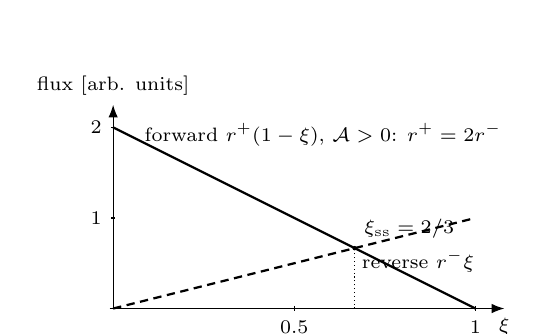
\begin{tikzpicture}[x=4.6cm,y=1.15cm]
\draw[-{Latex[length=1.6mm]}] (0,0) -- (0,2.25) node[above,font=\scriptsize] {flux [arb. units]};
\draw[-{Latex[length=1.6mm]}] (-0.01,0) -- (1.08,0) node[below,font=\scriptsize] {$\xi$};
\foreach \xx in {0.5,1} {\draw (\xx,0.03) -- (\xx,-0.03) node[below,font=\scriptsize] {\xx};}
\foreach \yy in {1,2} {\draw (0.005,\yy) -- (-0.005,\yy) node[left,font=\scriptsize] {\yy};}
% forward flux r+(1-xi), r+=2 when A>0, so decreases from 2 to 0
\draw[thick] (0,2) -- (1,0);
% reverse flux r-*xi, r-=1, increases from 0 to 1
\draw[thick,densely dashed] (0,0) -- (1,1);
% intersection: r+(1-xi)=r- xi => 2(1-xi)=xi => xi=2/3
\draw[densely dotted] (0.6667,0) -- (0.6667,0.6667);
\fill (0.6667,0.6667) circle (0.8pt) node[above right,font=\scriptsize] {$\xi_{\sstat}=2/3$};
\node[right,font=\scriptsize] at (0.06,1.92) {forward $r^+(1-\xi)$, $\mathcal{A}>0$: $r^+=2r^-$};
\node[right,font=\scriptsize] at (0.66,0.52) {reverse $r^-\xi$};
\end{tikzpicture}
\caption{정지점 유도(신규): 정방향 $r^+(1-\xi)$(감소 직선)과 역방향 $r^-\xi$(증가 직선)의 교점.
$\mathcal A>0$($r^+=2r^-$)이면 $\xi_{\sstat}=2/3$; $\mathcal A=0$ 이면 $1/2$ — 식~\eqref{eq:stationary}.
이 교점이 logistic 에서 정확히 복원된다.}
\label{fig:fluxcross}
\end{figure}

\textbf{(c) 구동력 대입.} $\mathcal A_j = sF(V-U_j) - \Omega_j(1-2\xi_j)$ 이나, 이상 극한($\Omega=0$)에서
$\mathcal A_j = sF(V_n-U_j)$ 를 식~\eqref{eq:stationary} 에 대입하면
\begin{equation}
\frac{\xi_\eq}{1-\xi_\eq} = e^{sF(V-U)/RT}.
\label{eq:logitsolve}
\end{equation}

\textbf{(d) logistic 닫힘.} $\xi_\eq$ 에 대해 풀면(분자·분모를 $e^{sF(V-U)/RT}$ 로 나눔)
\begin{equation}
\xi_\eq = \frac{1}{1+e^{-sF(V-U)/RT}} = \frac{1}{1+e^{-\sigma_d(V-U)/w}},
\end{equation}
$s=\sigma_d$, $w=RT/F$ 를 넣고 다중도 $n_j$ 를 넣어 일반화하면

\begin{equation}
\boxed{\;\xi_{\eq,j}(V,T)=\frac{1}{1+\exp\!\big[-\sigma_d(V-U_j^{\,d})/w_j\big]}\;,\qquad
w_j=\frac{n_jRT}{F}\;.}
\label{eq:xieq}
\end{equation}
이것이 \code{func\_ksi\_eq(T, V\_n, U, n, s)} 다.

\begin{signbox}
\textbf{부호.} 방전 $\sigma_d=+1$: $V\!\uparrow\Rightarrow z\!\uparrow\Rightarrow\xi_\eq\!\uparrow$ —
전위를 올리면 탈리튬화 진행이 는다(규약 일치). 극한 — $V\gg U_j^{\,d}\Rightarrow\xi_\eq\to1$,
$V=U_j^{\,d}\Rightarrow\tfrac12$.
\end{signbox}

\begin{figure}[t]
\centering
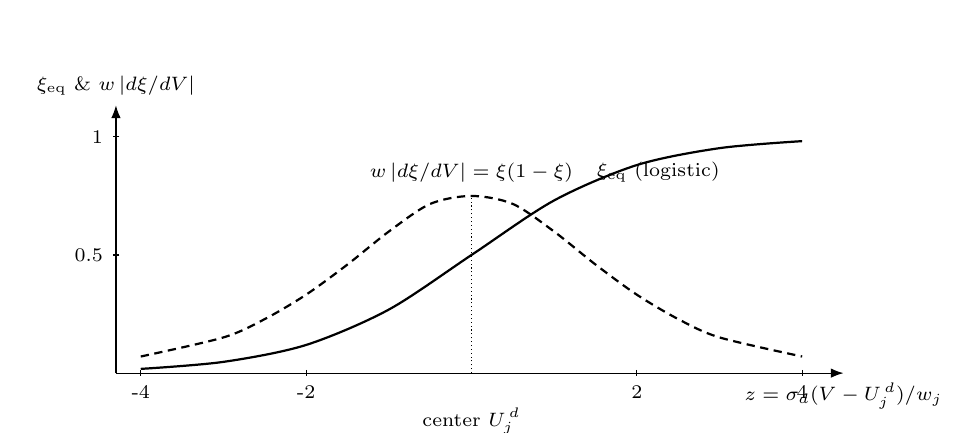
\begin{tikzpicture}[x=1.05cm,y=1.0cm]
\draw[-{Latex[length=1.6mm]}] (-4.3,0) -- (4.5,0) node[below,font=\scriptsize] {$z=\sigma_d(V-U_j^{\,d})/w_j$};
\draw[-{Latex[length=1.6mm]}] (-4.3,0) -- (-4.3,3.4) node[above,font=\scriptsize] {$\xi_\eq$ \&\ $w\,|d\xi/dV|$};
\foreach \xx in {-4,-2,2,4} {\draw (\xx,0.04) -- (\xx,-0.04) node[below,font=\scriptsize] {\xx};}
\draw (-4.26,3.0) -- (-4.34,3.0) node[left,font=\scriptsize] {1};
\draw (-4.26,1.5) -- (-4.34,1.5) node[left,font=\scriptsize] {0.5};
\draw[thick] plot[smooth] coordinates {(-4,0.0537) (-3,0.1429) (-2,0.3577) (-1,0.8068) (0,1.5) (1,2.1932) (2,2.6423) (3,2.8571) (4,2.9463)};
\node[right,font=\scriptsize] at (1.4,2.55) {$\xi_\eq$ (logistic)};
\draw[densely dashed,thick] plot[smooth] coordinates {(-4,0.211) (-3,0.4534) (-2.5,0.6864) (-2,0.9963) (-1.5,1.3792) (-1,1.7976) (-0.5,2.1487) (0,2.25) (0.5,2.1487) (1,1.7976) (1.5,1.3792) (2,0.9963) (2.5,0.6864) (3,0.4534) (4,0.211)};
\node[font=\scriptsize] at (0,2.55) {$w\,|d\xi/dV|=\xi(1-\xi)$};
\draw[densely dotted] (0,0)--(0,2.25);
\node[below,font=\scriptsize] at (0,-0.32) {center $U_j^{\,d}$};
\end{tikzpicture}
\caption{평형 점유와 그 미분(v7-11 유래). 실선 $=\xi_\eq$ logistic(식~\eqref{eq:xieq}), 파선 $=$ 폭으로 규격화한 미분
$w_j|d\xi_\eq/dV|=\xi_\eq(1-\xi_\eq)$ — 중심에서 최대 $\tfrac14$ 인 종 모양.}
\label{fig:logistic}
\end{figure}

% ====================================================================
\section{평형 peak — $|I|\to0$ 기준선 (N6)}\label{sec:eqpeak}
% ====================================================================
코드는 평형 점유에서 곧바로 평형 peak 모양 $\xi_\eq(1-\xi_\eq)/w$ 를 만든다.

\textbf{(a) 출발: 전하 보존식.} 관측 $\dd Q/\dd V$ 는 전하 보존식
$Q_\cell q = Q_\bg(V_n) + \sum_j Q_j\xi_j$ 를 궤적 $q$ 로 미분해
\begin{equation}
\frac{\dd Q}{\dd V_n} = C_\bg + \sum_j Q_j\frac{\dd\xi_j}{\dd V_n}
\label{eq:dqdv_general}
\end{equation}
로 닫힌다.

\textbf{(b) logistic 미분.} 평형 추종이면 $\dd\xi_j/\dd V_n$ 에 평형 기울기가 들어간다.
logistic 항등식 $\dd\xi_\eq/\dd z = \xi_\eq(1-\xi_\eq)$ 에 연쇄율 $\dd z/\dd V = \sigma_d/w_j$ 를 곱하면
\begin{equation}
\frac{\dd\xi_{\eq,j}}{\dd V} = \frac{\sigma_d\,\xi_{\eq,j}(1-\xi_{\eq,j})}{w_j}.
\label{eq:dxidV}
\end{equation}

\textbf{(c) 평형 peak 닫힘.} $|\dd\xi/\dd V|$ 는 부호 불변이므로
\begin{equation}
\boxed{\;\Bigl(\frac{\dd Q}{\dd V}\Bigr)^\eq_j
=Q_j\,\frac{\xi_{\eq,j}(1-\xi_{\eq,j})}{w_j}
=Q_j\,\Bigl|\frac{\dd\xi_{\eq,j}}{\dd V}\Bigr|\;.}
\label{eq:eqpeak}
\end{equation}
이것이 코드의 \code{peak\_shape = ksi\_eq * (1 - ksi\_eq) / w} 다.
세 양 — 위치 $=$ 중심 $U_j^{\,d}$, 순높이 $=Q_j/(4w_j)$($\xi=\tfrac12$ 에서 $\xi(1-\xi)=\tfrac14$),
면적 $=Q_j$ — 가 이 한 식에서 읽힌다.

% ====================================================================
\section{동역학 지연 길이 $L_V$ (N7)}\label{sec:lag}
% ====================================================================
유한 전류에서는 평형 목표 $\xi_\eq$ 를 점유가 즉시 따라가지 못하고 뒤처진다. 이 절은 지연 ODE 유도,
적분인자 해, Eyring 속도 상수, $L_q$ 와 $L_V$ 닫힘까지 전 사슬을 전개한다.

\subsection{지연 ODE와 적분인자 일반해}

\textbf{(a) 출발: 운동방정식을 용량축으로.} 정전류에서 $\dd q/\dd t = |I|/Q_\cell$ 이고,
$r_j \equiv \xi_{\eq,j}-\xi_j$ 라 두면 식~\eqref{eq:relax} 로부터
\begin{equation}
\frac{\dd\xi_j}{\dd t} = k_j(\xi_{\eq,j}-\xi_j) = k_j r_j.
\label{eq:dxidt}
\end{equation}
$\dd r_j/\dd t = \dd\xi_{\eq,j}/\dd t - \dd\xi_j/\dd t$ 이므로 양변을 $\dd q/\dd t = |I|/Q_\cell$ 로 나누면

\textbf{(b) 지연 ODE.}
\begin{equation}
\frac{\dd r_j}{\dd q} = \frac{\dd\xi_{\eq,j}}{\dd q} - \frac{r_j}{L_{q,j}},
\qquad L_{q,j} = \frac{|I|}{Q_\cell\,k_j}.
\label{eq:Lq}
\end{equation}
$L_{q,j}$ 는 요구($|I|/Q_\cell$)와 공급($k_j$)의 비 그 자체다.

\textbf{(c) 적분인자 일반해.} 식~\eqref{eq:Lq} 는 1계 선형 ODE 다. 적분인자 $e^{q/L_{q,j}}$ 를 곱하면
\begin{equation}
\frac{\dd}{\dd q}\bigl[e^{q/L_{q,j}}r_j\bigr] = e^{q/L_{q,j}}\frac{\dd\xi_{\eq,j}}{\dd q}.
\label{eq:ifactor}
\end{equation}
$q_0$ 에서 $q$ 까지 적분하면
\begin{equation}
r_j(q) = r_j(q_0)e^{-(q-q_0)/L_{q,j}}
+ \int_{q_0}^q e^{-(q-q')/L_{q,j}}\frac{\dd\xi_{\eq,j}}{\dd q'}\,\dd q'.
\label{eq:gensol}
\end{equation}
초기 지연 $r_j(q_0)$ 은 지수적으로 사멸하고, 이후는 과거 목표 변화율을 지수 커널
$e^{-(q-q')/L_{q,j}}$ 로 가중한 기억의 합성곱이다 — 길이 $L_{q,j}$ 만큼의 최근 과거만 기억한다.

\subsection{Eyring 속도 상수와 완화 속도 $k_j$}

\textbf{(a) Eyring 전이상태 이론.} 전진 속도 상수는
\begin{equation}
k^+ = \frac{k_BT}{h}\exp\!\Bigl[-\frac{\Delta G_a^\eff - \chi_d\mathcal A}{RT}\Bigr]
\label{eq:eyring}
\end{equation}
($k_0 \equiv k_BT/h$: Eyring 사전지수 \cite{eyring1935},
$\Delta G_a^\eff = \Delta H_a^\eff - T\Delta S_a$, $\chi_d$: 방향별 전달 계수).

\textbf{(b) 완화 속도 — 정·역 합.} Detailed balance~\eqref{eq:db} 에서 $k^- = k^+ e^{-\mathcal A/RT}$ 이므로
\begin{equation}
k_j = k^+ + k^- = k^+\bigl(1+e^{-\mathcal A_j/RT}\bigr).
\label{eq:kuniv}
\end{equation}
이 괄호 인자가 역방향 기여의 전부다($\mathcal A\gg RT$ 에서 $1$ 로 죽고, 평형 근방에서 최대 $2$).

\subsection{컷 affinity $\mathcal A$ — 꼬리 시작점의 구동력}
$L_q$ 는 전이당 한 점(꼬리 컷점 $q_a$)에서 상수로 동결된다. 컷점은 원천 $\dd\xi_\eq/\dd q$ 가
정점의 약 $5\%$ 로 떨어지는 좌표이고, 그곳의 구동력 크기는 $z_\mathrm{cut}=4.357$($5\%$ 대응)로
\begin{equation}
\mathcal A=\min\!\big(z_\mathrm{cut}\,n_j\,RT,\;A_\mathrm{cap}\,RT\big),
\qquad z_\mathrm{cut}=4.357,\ A_\mathrm{cap}=4.0\ (\text{기본}).
\label{eq:Acut}
\end{equation}
부호의 핵심 — 크기만($\min$ 인자 모두 양수), 방향은 $\chi_d$ 와 $\Delta H_a^\eff$ 가 받는다.

\subsection{방향별 전달 계수와 유효 장벽}
전이상태가 정·역 장벽을 비대칭으로 가르는 분율 $\chi \in [0,1]$ 의 합-$1$ 제약에서
\begin{equation}
\chi_d=\begin{cases}\chi & \sigma_d\ge0\ (\text{방전})\\ 1-\chi & \sigma_d<0\ (\text{충전}).\end{cases}
\label{eq:chid}
\end{equation}
깊은 꼬리에서 방전은 $\xi\to1$, 충전은 $\xi\to0$ 거울이라 역방향 장벽의 상수 몫 $+\Omega$ 가
흡수되어
\begin{equation}
\boxed{\;\Delta H_{a,j}^\eff=\Delta H_{a,j}-\chi_d\,\Omega_j\;.}
\label{eq:dHeff}
\end{equation}

\subsection{$L_q$ 의 평가와 전압축 환산 $L_V$}
식~\eqref{eq:kuniv} 와 식~\eqref{eq:eyring} 를 식~\eqref{eq:Lq} 에 대입하면
$L_{q,j} = |I|/(Q_\cell k^+(1+e^{-\mathcal A/RT}))$ 이고, $k_0=k_BT/h$,
$\Delta G_a^\eff = \Delta H_a^\eff - T\Delta S_a$ 로 갈라 적으면
\begin{equation}
\boxed{\;L_{q,j}=\frac{T_*}{T}\,\frac{\exp\!\big[(\Delta H_{a,j}^\eff-T\Delta S_{a,j})/RT\big]}{1+e^{-\mathcal A/RT}}
\,e^{-\chi_d\mathcal A/RT},
\qquad T_*\equiv\frac{|I|\,h}{Q_\cell\,k_B}\;.}
\label{eq:Lqfull}
\end{equation}
코드는 이를 로그 합 \code{ln\_Lq = ln(T\_attempt/T) - ln(1+e\^{-A/RT}) + dG\_a/RT - x*A/RT} 로 평가한다.
전압축으로 옮기면 컷점 OCV 기울기를 곱해
\begin{equation}
\boxed{\;L_{V,j}=\Big|\frac{\dd V}{\dd q}\Big|_{q_a}\,L_{q,j}\;.}
\label{eq:LV}
\end{equation}

\textbf{부호의 핵심 — $\partial\ln L_q/\partial V$ 논의.} $\mathcal A$ 가 전이당 컷 상수라
운영상 실현 미분은 $\partial\ln L_q/\partial V = 0$ 이다. 부등식 $\partial\ln L_q/\partial V < 0$ 은
컷 규칙의 \emph{동기}로 읽어야 한다 — 만일 $\mathcal A$ 를 컷에 동결하지 않고 국소 구동력으로 두면
$V\!\uparrow\Rightarrow\mathcal A\!\uparrow\Rightarrow$ 유효 장벽$\downarrow\Rightarrow L_q\downarrow$.

\begin{codebox}
\textbf{N7 진행.} \code{n\_safe=|n\_j|} $\to$ $\mathcal A$(식~\eqref{eq:Acut}) $\to$
\code{(chi\_d, dH\_a\_use)=\_chi\_and\_dH\_eff(...)} $\to$
\code{L\_q=func\_L\_q(...,x=chi\_d,A=A)} (식~\eqref{eq:Lqfull}) $\to$ \code{L\_V=|dVdq\_qa|*L\_q}.
전이당 상수(대표 $T_\rep$)로 한 번 평가한다.
\end{codebox}

% ====================================================================
\section{인과 기억 꼬리와 충전 격자 역전 (N8)}\label{sec:tail}
% ====================================================================
$L_{V,j}$ 가 충분히 크면 코드는 평형 종 대신 인과 기억 꼬리를 만든다.
그림~\ref{fig:memorykernel} 이 지수 커널 합성곱의 구조를 보인다.

\subsection{지수 기억 — 이산형 저역통과}
일반해~\eqref{eq:gensol} 의 지수 커널을 이산 격자에서 근사하면, 한 칸당 감쇠
$\rho = \exp(-\Delta_\mathrm{grid}/L_V)$ 의 점화식
\begin{equation}
\xi_{\mathrm{lag},i}=\rho\,\xi_{\mathrm{lag},i-1}+(1-\rho)\,\xi_{\eq,i}
\label{eq:lowpass}
\end{equation}
이다. 코드 \code{\_causal\_lowpass} 가 이를 \code{scipy.signal.lfilter} 계수
$[1-\rho]/[1,-\rho]$ 로 평가한다.

\begin{figure}[t]
\centering
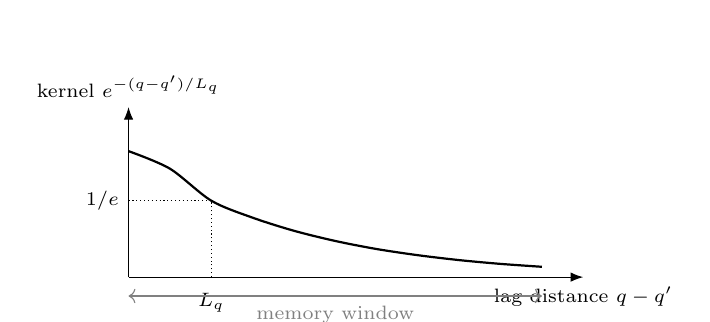
\begin{tikzpicture}[x=1.05cm,y=1.6cm]
\draw[-{Latex[length=1.6mm]}] (0,0) -- (5.5,0) node[below,font=\scriptsize] {lag distance $q-q'$};
\draw[-{Latex[length=1.6mm]}] (0,0) -- (0,1.35) node[above,font=\scriptsize] {kernel $e^{-(q-q')/L_q}$};
\draw[thick] plot[smooth] coordinates {(0,1.0)(0.5,0.861)(1.0,0.607)(1.5,0.472)(2.0,0.368)
  (2.5,0.287)(3.0,0.223)(3.5,0.174)(4.0,0.135)(4.5,0.105)(5.0,0.082)};
\draw[densely dotted] (1.0,0)--(1.0,0.607);
\draw[densely dotted] (0,0.607)--(1.0,0.607);
\node[below,font=\scriptsize] at (1.0,-0.05) {$L_q$};
\node[left,font=\scriptsize] at (0,0.607) {$1/e$};
\draw[<->,gray] (0,-0.15)--(5.0,-0.15) node[midway,below,font=\scriptsize] {memory window};
\end{tikzpicture}
\caption{지수 기억 커널(신규). 지연 ODE~\eqref{eq:gensol} 의 일반해가 갖는 지수 커널
$e^{-(q-q')/L_q}$ 의 모양. $L_q$ 에서 $1/e$ 로 감쇠 — 길이 $L_q$ 만큼의 최근 과거만 기억한다.
이산화하면 식~\eqref{eq:lowpass} 의 저역통과가 된다.}
\label{fig:memorykernel}
\end{figure}

\subsection{peak 모양 — 평형에서 지연을 뺀 것}
\begin{equation}
\boxed{\;\text{peak\_shape}=\frac{\xi_{\eq}-\xi_{\mathrm{lag}}}{L_{V,j}}\;.}
\label{eq:peakshape}
\end{equation}
$L_V$ 가 작으면 $\xi_\mathrm{lag}\approx\xi_\eq$ (1칸 이동)라 이산 미분 $\to\dd\xi_\eq/\dd V$ 의
종으로 환원되어 평형 peak~\eqref{eq:eqpeak} 로 돌아간다:
\begin{equation}
\text{peak\_shape}=
\begin{cases}
\xi_\eq(1-\xi_\eq)/w & L_{V,j}<\nu\,\Delta_\mathrm{grid}\ \text{(평형 종)}\\[2pt]
(\xi_\eq-\xi_\mathrm{lag})/L_{V,j} & \text{그 외 (꼬리 종)},
\end{cases}
\label{eq:branch}
\end{equation}
$\nu=\code{min\_lag\_grid\_steps}=2$ 다.

\subsection{★충전 격자 역전 — 인과 방향}
인과 합성곱은 ``진행 방향의 과거''를 기억한다. 방전($\sigma_d=+1$)은 $V$ 증가 방향이라
격자 오름차순이 곧 시간 순서이고, 저역통과를 그대로 적용한다. 충전($\sigma_d=-1$)은 $V$ 감소 방향 —
격자 오름차순의 \emph{역}이 시간 순서다. 따라서
\begin{equation}
\xi_\mathrm{lag}=
\begin{cases}
\code{causal\_lowpass}(\xi_\eq) & \sigma_d\ge0\ (\text{방전})\\[2pt]
\code{causal\_lowpass}(\xi_\eq[::-1])[::-1] & \sigma_d<0\ (\text{충전}).
\end{cases}
\label{eq:reversal}
\end{equation}
이 역전이 없으면 충전 꼬리가 미래를 기억하는 비인과 신호가 되어 peak 가 엉뚱한 쪽으로 번진다.

\begin{figure}[t]
\centering
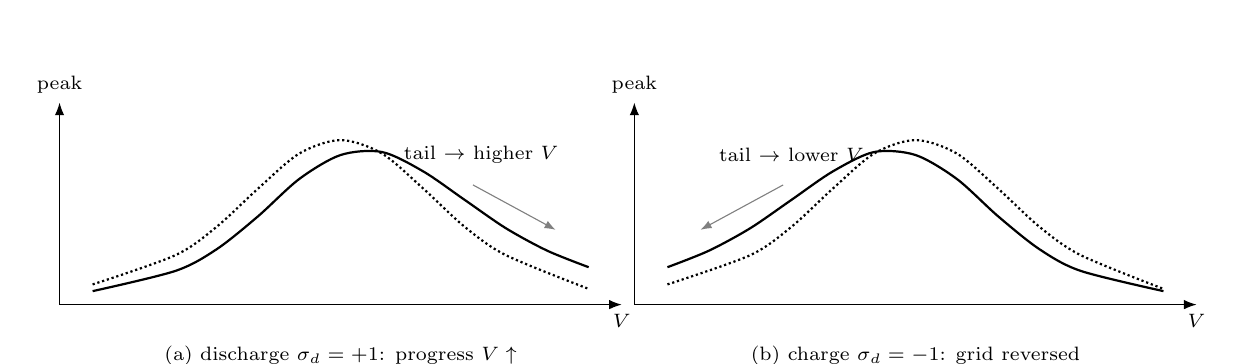
\begin{tikzpicture}[x=1.05cm,y=0.95cm]
% discharge panel (left)
\begin{scope}
\draw[-{Latex[length=1.6mm]}] (-3.4,0) -- (3.4,0) node[below,font=\scriptsize] {$V$};
\draw[-{Latex[length=1.6mm]}] (-3.4,0) -- (-3.4,2.7) node[above,font=\scriptsize] {peak};
\draw[densely dotted,thick] plot[smooth] coordinates {(-3,0.27) (-2,0.66) (-1.5,1.04) (-1,1.55) (-0.5,2.02) (0,2.2) (0.5,2.02) (1,1.55) (1.5,1.04) (2,0.66) (3,0.21)};
\draw[thick] plot[smooth] coordinates {(-3,0.18) (-2,0.45) (-1.5,0.74) (-1,1.18) (-0.5,1.68) (0,2.0) (0.5,2.04) (1,1.78) (1.5,1.4) (2,1.02) (2.5,0.72) (3,0.5)};
\draw[-{Latex[length=1.4mm]},gray] (1.6,1.6)--(2.6,1.0);
\node[font=\scriptsize] at (1.7,2.0) {tail $\to$ higher $V$};
\node[font=\scriptsize,below] at (0,-0.42) {(a) discharge $\sigma_d=+1$: progress $V\uparrow$};
\end{scope}
% charge panel (right)
\begin{scope}[xshift=7.3cm]
\draw[-{Latex[length=1.6mm]}] (-3.4,0) -- (3.4,0) node[below,font=\scriptsize] {$V$};
\draw[-{Latex[length=1.6mm]}] (-3.4,0) -- (-3.4,2.7) node[above,font=\scriptsize] {peak};
\draw[densely dotted,thick] plot[smooth] coordinates {(-3,0.27) (-2,0.66) (-1.5,1.04) (-1,1.55) (-0.5,2.02) (0,2.2) (0.5,2.02) (1,1.55) (1.5,1.04) (2,0.66) (3,0.21)};
\draw[thick] plot[smooth] coordinates {(-3,0.5) (-2.5,0.72) (-2,1.02) (-1.5,1.4) (-1,1.78) (-0.5,2.04) (0,2.0) (0.5,1.68) (1,1.18) (1.5,0.74) (2,0.45) (3,0.18)};
\draw[-{Latex[length=1.4mm]},gray] (-1.6,1.6)--(-2.6,1.0);
\node[font=\scriptsize] at (-1.5,2.0) {tail $\to$ lower $V$};
\node[font=\scriptsize,below] at (0,-0.42) {(b) charge $\sigma_d=-1$: grid reversed};
\end{scope}
\end{tikzpicture}
\caption{인과 꼬리의 방향(v7-11 유래, 개선). 점선 $=$ 평형 종. 실선 $=$ peak\_shape with tail.
(a) 방전은 꼬리가 높은 $V$ 쪽으로. (b) 충전은 격자를 뒤집어 필터($\xi[::-1]\cdots[::-1]$)해 꼬리가 낮은 $V$ 쪽 — 방전의 거울. 두 경우 모두 peak 는 양수.}
\label{fig:reversal}
\end{figure}

% ====================================================================
\section{합산과 역보간 (N9)}\label{sec:sum}
% ====================================================================
전이 루프가 각 전이의 peak\_shape 를 만들면, 코드는 용량 가중을 곱해 누적하고, 마지막에 내부 전위
격자로 역보간한다. 보존식 $Q_\cell q=Q_\bg+\sum_jQ_j\xi_j$ 가 $\sum_jQ_j\xi_j$ 꼴이라

\textbf{(a) 합산.}
\begin{equation}
\boxed{\;\frac{\dd Q}{\dd V}(V_n)\;=\;C_\bg\;+\;\sum_{j=1}^{N_p}Q_j\,
\bigl[\text{peak\_shape}_j\bigr]\;.}
\label{eq:sum}
\end{equation}
코드는 \code{dqdv\_work += tr['Q'] * peak\_shape} 로 누적하고,
\code{np.interp(V\_n, V\_work, dqdv\_work)} 로 되돌린다.

\subsection{staging 전이 초기값}
\begin{table}[t]
\centering
\renewcommand{\arraystretch}{1.25}
\caption{전이 초기값 \code{GRAPHITE\_STAGING\_LIT}(4건). 피팅 출발점.}
\label{tab:staging}
\begin{tabular}{l c c c c c c c}
\toprule
stage & $U$ [V] & $\Delta H_\rxn$ & $\Delta S_\rxn$ & $Q$ & $\Omega$ & $\Delta H_a$ & $|\dd V/\dd q|_{q_a}$ \\
 &  & [J/mol] & [J/(mol\,K)] & [$Q_\cell$] & [J/mol] & [J/mol] & [V] \\
\midrule
$4\!\to\!3$   & 0.210 & $-11700$ & $+29.0$ & 0.10 & 6000  & 48000 & 0.30 \\
$3\!\to\!2\mathrm L$ & 0.140 & $-13500$ & $0.0$   & 0.12 & 8000  & 46000 & 0.30 \\
$2\mathrm L\!\to\!2$ & 0.120 & $-13100$ & $-5.0$  & 0.25 & 10000 & 44000 & 0.30 \\
$2\!\to\!1$   & 0.085 & $-13000$ & $-16.0$ & 0.50 & 13000 & 40000 & 0.30 \\
\bottomrule
\end{tabular}
\end{table}

\subsection{전체 입력 인자와 기본값}
\begin{table}[t]
\centering\footnotesize
\renewcommand{\arraystretch}{1.18}
\caption{전체 입력 인자(코드 식별자)와 기본값.}
\label{tab:inputs}
\begin{tabular}{l l l l}
\toprule
인자(코드) & 자리 & 기본값 & 역할(식) \\
\midrule
\multicolumn{4}{l}{\emph{— 전이 dict 키(전이별) —}}\\
\code{U} 또는 (\code{dH\_rxn},\code{dS\_rxn}) & 전이 & --- & 평형 중심 $U_j(T)$ (\eqref{eq:Uj}) \\
\code{w} 또는 \code{n} & 전이 & --- / $1$ & 폭 $w_j=n_jRT/F$ (\eqref{eq:wbase}) \\
\code{Q} & 전이 & --- & 용량 가중 \\
\code{Omega},\code{gamma} & 전이 & $0$,\,$0$ & 상호작용$\cdot$분기 (\eqref{eq:dUhys}\eqref{eq:Ubranch}) \\
\code{h\_eta} & 전이 & $1.0$ & 부분 cycle 분기 인자 \\
\code{dH\_a},\code{dS\_a} & 전이 & --- / $0$ & 활성화(꼬리, \eqref{eq:Lqfull}) \\
\code{dVdq\_qa} & 전이 & $0$ & 컷 OCV 기울기 (\eqref{eq:LV}) \\
\code{L\_V} & 전이 & --- & 직접 지연 길이 \\
\code{z\_cut},\code{A\_cap\_RT} & 전이/공통 & $4.357$,\,$4.0$ & 컷 affinity (\eqref{eq:Acut}) \\
\multicolumn{4}{l}{\emph{— 생성자 인자(모델 공통) —}}\\
\code{x}/\code{chi} & 공통 & $0.5$ & 전달 계수 $\chi_d$ (\eqref{eq:chid}) \\
\code{Rn} & 공통 & $0.0$ & 분극 저항 (\eqref{eq:vn}) \\
\code{Cbg} & 공통 & $0.0$ & 배경 $C_\bg$ \\
\code{grid\_pad\_lo/hi},\,\code{n\_work\_min} & 공통 & $0.15$,\,$2048$ & 작업 격자 (\eqref{eq:vwork}) \\
\code{min\_lag\_grid\_steps} & 공통 & $2.0$ & 꼬리/평형 전환 (\eqref{eq:branch}) \\
\bottomrule
\end{tabular}
\end{table}

\begin{keybox}
\textbf{이 문건만으로 한 곡선 재현(6단계).}
(1) 표~\ref{tab:staging} 의 4 전이로 \code{transitions} 구성.
(2) 실험조건 $\sigma_d$, $|I|$, $T$, $R_n$ 설정 $\to$ $V_n$(\eqref{eq:vn}), $V_\work$(\eqref{eq:vwork}).
(3) 전이마다 $U_j(T)$(\eqref{eq:Uj}) $\to$ 분기 중심(\eqref{eq:center}) $\to$ $w_j$(\eqref{eq:wbase}) $\to$ $\xi_\eq$(\eqref{eq:xieq}).
(4) 지연 길이: $\mathcal A$(\eqref{eq:Acut}) $\to$ $\chi_d,\Delta H_a^\eff$(\eqref{eq:chid}\eqref{eq:dHeff}) $\to$ $L_q$(\eqref{eq:Lqfull}) $\to$ $L_V$(\eqref{eq:LV}).
(5) peak\_shape: $L_V<2\Delta_\mathrm{grid}$ 면 평형 종(\eqref{eq:eqpeak}), 아니면 인과 꼬리(\eqref{eq:peakshape}, 충전 역전 \eqref{eq:reversal}).
(6) 용량 가중 합산 후 $V_n$ 으로 역보간(\eqref{eq:sum}).
\end{keybox}

\begin{table}[t]
\centering
\renewcommand{\arraystretch}{1.3}
\caption{노드 $\leftrightarrow$ 식 $\leftrightarrow$ 코드 식별자 매핑.}
\label{tab:nodemap}
\begin{tabular}{l l l l}
\toprule
노드 & 물리식 & 본 문건 식 & 코드 식별자 \\
\midrule
N0 & $\sigma_d,|I|$ & \eqref{eq:n0map} & \code{curve},\code{\_direction\_to\_sigma} \\
N1 & $V_n=V_\app-\sigma_d|I|R_n$ & \eqref{eq:vn} & \code{dqdv} L412 \\
N2 & $U_j(T)=(-\Delta H+T\Delta S)/F$ & \eqref{eq:Uj} & \code{func\_U\_j} \\
N3 & $\Delta U_j^\hys$, $U_j^{\,d}$ & \eqref{eq:dUhys},\eqref{eq:Ubranch} & \code{func\_dU\_hys},\code{func\_U\_branch} \\
N4 & $w_j=n_jRT/F$ & \eqref{eq:wbase}(\eqref{eq:weff}) & \code{func\_w},\code{func\_w\_eff} \\
N5 & $\xi_\eq=\mathrm{logistic}[\sigma_d(V-U^d)/w]$ & \eqref{eq:xieq} & \code{func\_ksi\_eq} \\
N6 & $Q_j\xi_\eq(1-\xi_\eq)/w$ & \eqref{eq:eqpeak} & \code{equilibrium} \\
N7 & $\mathcal A,\chi_d,\Delta H_a^\eff,L_q,L_V$ & \eqref{eq:Acut}--\eqref{eq:LV} & \code{\_resolve\_lag\_length},\code{func\_L\_q} \\
N8 & $(\xi_\eq-\xi_\mathrm{lag})/L_V$, 역전 & \eqref{eq:peakshape},\eqref{eq:reversal} & \code{\_causal\_lowpass} \\
N9 & $C_\bg+\sum_jQ_j[\cdot]$ & \eqref{eq:sum} & \code{dqdv\_work},\code{np.interp} \\
\bottomrule
\end{tabular}
\end{table}

% ====================================================================
\section{부호 사슬 전수 검산}\label{sec:signcheck}
% ====================================================================
브리프 §8 의 부호 체크리스트를 전건 확인한다. 기준 명제 = \emph{방전 시
$V\!\uparrow\Rightarrow$ 탈리튬화$\uparrow$, 충전 $\dd Q/\dd V$ 는 방전의 거울(양수)}.

\begin{enumerate}[label=\textbf{S\arabic*.},leftmargin=2.6em,itemsep=2pt]
\item \textbf{$U_j(T)=(-\Delta H+T\Delta S)/F$, $\Delta G=-FU$.} 식~\eqref{eq:Uj}$\cdot$\eqref{eq:eqcond}.
$\Delta H_\rxn<0$(발열)이면 $-\Delta H_\rxn>0$ 이 중심을 올린다. $\Delta G_j=-sFU_j$ 부호 일치. $\checkmark$
\item \textbf{$\xi_\eq=\mathrm{logistic}[\sigma_d(V-U)/w]$.} 식~\eqref{eq:xieq}. 방전 $\sigma_d=+1$ 에서
$V\!\uparrow\Rightarrow\xi_\eq\!\uparrow$. $\checkmark$
\item \textbf{$d\xi/dV=\sigma_d\,\xi(1-\xi)/w$, peak 양수.} 식~\eqref{eq:eqpeak}. peak 모양 $=|\dd\xi/\dd V|=
\xi(1-\xi)/w\ge0$, 방향 불변. $\checkmark$
\item \textbf{$\Delta U_\hys\ge0$, $\Omega\le2RT\to0$; 분기 중심 $\pm\tfrac12\sigma_d$.} 식~\eqref{eq:dUhys}$\cdot$
\eqref{eq:Ubranch}. 극대 $>$ 극소라 $\ge0$; $u_j\to0$ 에서 $0$; 방전 $+$/충전 $-$ 라 $U^\dis>U^\chg$. $\checkmark$
\item \textbf{$\chi_d$: 방전 $\chi$/충전 $1-\chi$; $\Delta H_a^\eff=\Delta H_a-\chi_d\Omega$.} 식~\eqref{eq:chid}$\cdot$
\eqref{eq:dHeff}. 합-$1$ 거울 대칭. $\checkmark$
\item \textbf{$\partial\ln L_q/\partial V<0$ (물리적 동기).} $\mathcal A$ 가 컷 상수라 운영상 실현 미분은
$\partial\ln L_q/\partial V=0$. 부등식은 컷 규칙의 동기. 자기모순 없음. $\checkmark$
\item \textbf{꼬리: 충전 격자 역전; 충전 $\dd Q/\dd V$ 방전 거울(양수).} 식~\eqref{eq:reversal}.
peak\_shape $=(\xi_\eq-\xi_\mathrm{lag})/L_V>0$. $\checkmark$
\item \textbf{분극 $V_n=V_\app-\sigma_d|I|R_n$.} 식~\eqref{eq:vn}. 방전 시 측정 $>$ 내부. $\checkmark$
\end{enumerate}
전건이 기준 명제와 정합한다 — 부호 결함 $0$.

\begin{verifybox}
\textbf{부호 회귀 self-test.}
\begin{enumerate}[label=\textbf{R\arabic*.},leftmargin=2.6em,itemsep=1pt]
\item \textbf{히스 분기 방향.} $\Omega=12000$ J/mol, $\gamma=1$ 에서
$u=\sqrt{1-2RT/\Omega}=\sqrt{1-4958/12000}=0.766$,
$\Delta U^\hys=\frac{2}{F}[\Omega u-2RT\,\mathrm{artanh}\,u]=86.7$ mV $>0$.
방전 peak 위치 $-$ 충전 peak 위치 $= +86.7$ mV $>0$ — 기준 명제 일치.
\item \textbf{히스 문턱.} $\Omega=2RT=4958$ J/mol 에서 $u=0$,
$\Delta U^\hys=0.0$ mV — $\Omega\le2RT$ 분기가 정확히 $0$ 으로 연속.
\item \textbf{$|I|\!\to\!0$ 환원·방향 불변.} $|I|\to0$ 에서 $L_V\propto|I|\to0$,
peak 가 평형 종 $\xi_\eq(1-\xi_\eq)/w$ 로 떨어지고 $\sigma_d$ 불변.
\item \textbf{$L_q$ 동결 vs 부등식.} $\mathcal A$ 가 전이당 상수라 $\partial\ln L_q/\partial V=0$,
부등식은 동기(자기모순 $0$).
\end{enumerate}
\end{verifybox}

% ====================================================================
\begin{thebibliography}{9}
\bibitem{dahn1991} J. R. Dahn, ``Phase diagram of Li$_x$C$_6$,'' \emph{Phys. Rev. B} \textbf{44}, 9170 (1991).
\bibitem{ohzuku1993} T. Ohzuku, Y. Iwakoshi, K. Sawai, ``Formation of Lithium-Graphite Intercalation Compounds,'' \emph{J. Electrochem. Soc.} \textbf{140}, 2490 (1993).
\bibitem{bazant2013} M. Z. Bazant, ``Theory of Chemical Kinetics and Charge Transfer based on Nonequilibrium Thermodynamics,'' \emph{Acc. Chem. Res.} \textbf{46}, 1144 (2013).
\bibitem{eyring1935} H. Eyring, ``The Activated Complex in Chemical Reactions,'' \emph{J. Chem. Phys.} \textbf{3}, 107 (1935).
\bibitem{dreyer2010} W. Dreyer \emph{et al.}, ``The thermodynamic origin of hysteresis in insertion batteries,'' \emph{Nature Materials} \textbf{9}, 448 (2010).
\bibitem{bloom2005} I. Bloom \emph{et al.}, ``Differential voltage analyses of high-power, lithium-ion cells,'' \emph{J. Power Sources} \textbf{139}, 295 (2005).
\bibitem{dubarry2012} M. Dubarry, C. Truchot, B. Y. Liaw, ``Synthesize battery degradation modes,'' \emph{J. Power Sources} \textbf{219}, 204 (2012).
\end{thebibliography}

\end{document}
